\chapter{The Executable Object Command Language (XOCL)}

The super-language XMF runs programs. XMF can run many different programming
languages, some interleaved, some completely separate. The basic language
provided with XMF is called XOCL - the executable object command language.
XOCL is very high-level and provides many features that make developing
applications easy. In addition to application development, XOCL is
intended for language engineering. You are likely to be using XMF
for its language engineering facilities and as such are going to use
XOCL to write languages. In order for your languages to do something
you are likely to link them to XOCL in some way, by translating them
to XOCL or by writing an language interpreter for them in XOCL.

This chapter describes the basic features of the XOCL language. XOCL
executes in terms of the concepts that were introduced in the previous
chapter. In order to ensure that we practice what we preach, XOCL
is completely implemented in XOCL: it has a grammar written in XOCL,
a compiler written in XOCL and an interpreter written in XOCL. That
property should not concern us when introducing the language, but
should give you confidence that XOCL is a good language for doing
language engineering!


\section{Working With Basic Elements}

The simplest components of XOCL are constants (notice that comments
follow // on a single line or within /{*} and {*}/ over multiple lines
as in Java):

\begin{lstlisting}
10             // An integer.
3.145          // A float.
true           // A boolean.
"Hello World"  // A string.
\end{lstlisting}
Basic operators are: not, (unary)-, + (binary)-, {*}, /, <, <=, >,
>=, =, and, or, andthen, orelse. Here is an operation definition in
XOCL: 

\begin{lstlisting}
context Root
  @Operation fact(n)
    if n = 0
    then 1
    else n * fact(n - 1)
    end
  end
\end{lstlisting}
The operator is named fact, takes a single argument n and is defined
in the global context Root which means that the name fact is available
everywhere. The argument n is local to the body of fact. All constructs
in XOCL return a value; the if-expression returns 1 or calls fact
again to return a value. If you want to follow along with a live XMF
system then you can type the definitions into a file and load them
and run the examples. To keep things short, we have omitted information
that would be in a source file. The file would actually look as follows:

\begin{lstlisting}
parserImport XOCL;

context Root
  @Operation fact(n)
    if n = 0
    then 1
    else n * fact(n - 1)
    end
  end
\end{lstlisting}
To load this into your system you would do the following:

\begin{center}
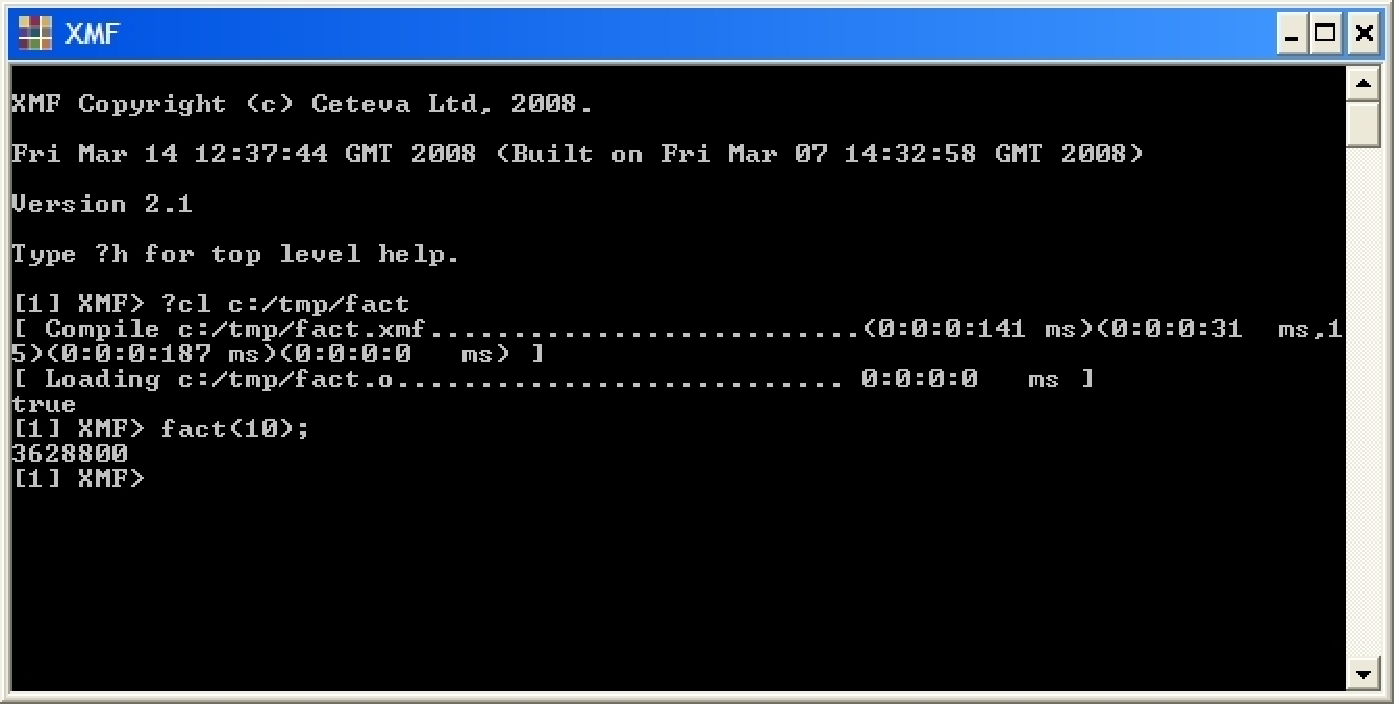
\includegraphics[width=15cm]{XMF/XOCL/Images/FactLoad.pdf}
\end{center}

Another example of a global operation definition is gcd below that
computes the greatest common divisor for a pair of positive integers.
The example shows that operations can optionally have argument and
return types:

\begin{lstlisting}
context Root
  @Operation gcd(m:Integer,n:Integer):Integer
    if m = n 
    then n
    elseif m > n 
    then gcd(m-n,n)
    else gcd(m,n-m)
    end
  end
\end{lstlisting}
Integers are arbitrary precision in XMF. 

The operators 'and' and 'or' are overloaded to perform bit comparison
when supplied with integers. The operators lsh and rsh are defined
on integers. They take the number of bits to shift left and right
respectively. The following operation adds up the number of bits in
an integer:

\begin{lstlisting}
context Root
  @Operation addBits(n:Integer):Integer
    if n = 0 or n < 0
    then 0
    else (n and 1) + (addBits(n.rsh(1)))
    end
  end
\end{lstlisting}
In addition, integers support the following operators: mod, abs, bit,
max, min and byte. XOCL supports floating point numbers. All numeric
operators described above are defined for floating point numbers.
In general integers and floats can be mixed in expressions and the
integer is translated to the equivalent float. You can construct a
float using the constructor Float so that 3.14 is created by Float(''3'',''14'').
Floats are translated to integers by the operations round (upwards)
and floor (downwards).

Integer division is performed by the operation div and floating point
division is performed by the infix operator / (translating integers
to floats as necessary). The operators sqrt, sin and cos are defined
for floats. 

All values in XMF support the operation 'of' that returns the most
specific class of the receiver. A value can be asked whether it is
of a given class using the operator isKindOf. Classes can be compared
using inheritsFrom where a class is considered to inherit from itself.
We could define isKindOf as:

\begin{lstlisting}
context Element
  @Operation isKindOf(type:Classifier):Boolean
    self.of().inheritsFrom(type)
  end
\end{lstlisting}
The distinguished value null, of type Null, is special in that it
returns true when asked whether it isKindOf any class. It is used
as the default value for all non-basic classes in XMF.

XMF strings are of type String. The following operation wraps the
string \char`\"{}The\char`\"{} and \char`\"{}.\char`\"{} around a
supplied string:

\begin{lstlisting}
context Root
  @Operation makeSentence(noun:String):String
    "The " + noun + "."
  end
\end{lstlisting}
Strings are sequences of characters indexed starting from 0. Equality
of strings is defined by = on a character by character comparison.
Characters are represented as integer ASCII codes. The following operation
checks whether a string starts with an upper case char:

\begin{lstlisting}
context Root
  @Operation startsUpperCase(s:String):Boolean
    if s->size > 0
    then
      let c = s->at(0)
      in "A"->at(0) <= c and c <= "Z"->at(0)
      end
    else false
    end
  end
\end{lstlisting}
Strings can be compared using <, <=, > and >= in which case the usual
lexicographic ordering applies.

Since strings are compared on a character by character basis this
makes string comparison relatively inefficient when performing many
comparisons. Strings are often used as the keys in lookup tables (for
example as the names of named elements). In order to speed up comparison,
XMF provides a specialization of String called Symbol. A symbol is
the same as a string except that two symbols with the same sequence
of characters have the same identity. Comparison of symbols by identity
rather than character by character is much more efficient. A string
s can be converted into a symbol by Symbol(s).

Any value can be converted into a string using the operation toString.
To get the string representation of a number for example: 100.toString()).


\section{Tables}

A table is used to associate keys with values. A table has operations
to add associations between keys and values and lookup a given key.
A table is created using the Table constructor supplying a single
argument that indicates the approximate number of elements to be stored
in the table. Suppose that a library maintains records on borrowers:

\begin{lstlisting}
context Root
  @Class Library
    @Attribute borrowers : Table = Table(100) end
  end
\end{lstlisting}
A new borrower is added by supplying the id, name and address. When
the new borrower is added we check that no borrower has been allocated
the same id. If the id is not already in use then we register the
new borrower by associating the id with a borrower record in the table:

\begin{lstlisting}
context Library
  @Operation newBorrower(id:String,name:String,address:String)
    if not borrowers.hasKey(id)
    then
      let borrower = Borrower(id,name,address)
      in borrowers.put(id,borrower)
      end
    else self.error("Borrower with id = " + id + " already exists.")
    end
  end
\end{lstlisting}
The library also provides an operation that gets a borrower record:

\begin{lstlisting}
context Library
  @Operation getBorrower(id:String):Borrower
    if borrowers.hasKey(id)
    then borrowers.get(id)
    else self.error("No borrower with id = " + id)
    end
  end
\end{lstlisting}
Tables provide operations to get all the keys and all the values:

\begin{lstlisting}
context Library
  @Operation idsInUse():Set(String)
    borrowers.keys()
  end
context Library
  @Operation allBorrowers():Set(Borrower)
    borrowers.values()
  end
\end{lstlisting}
\begin{itemize}
\item Constants, BinExp, Negate
\item Operations, Imports, Apply
\end{itemize}

\section{Sets}

A set is an unordered collection of elements. The elements of a set
need not all be of the same type. When T is the type of each element
of the set then the set is of type Set(T). Operations are provided
to add and remove elements from sets and to combine sets. Sets can
be used in iterate expressions.

Sets are created by evaluating a set expression of the form: Set\{x,y,z,...\}
where x, y, z etc are element expressions. For example:

\begin{lstlisting}
Set{1,true,Set{"a","b","c"},Borrower("1","Fred","3 The Cuttings")}
\end{lstlisting}
The expression Set\{\} produces the empty set. A set is unordered.
An element can be selected at random from a non-empty set by performing
S->sel. A set is empty when S->isEmpty produces true (or when it is
= to Set\{\}). An element e is added to a set by S->including(e) and
removed from a set by S->excluding(e). The union of two sets is produced
by S1 + S2 and the difference is constructed by S1 - S2. An element
is contained in a set when S->includes(e).

Suppose that the set operation includes was not provided as part of
XOCL. It could be defined by:

\begin{lstlisting}
context Set(Element)
  @Operation includes(e:Element):Boolean
    if self->isEmpty
    then false
    else 
      let x = self->sel
      in if x = e
         then true
         else self->excluding(x)->includes(e)
         end
      end
    end
  end
\end{lstlisting}
\section{Sequences}

A sequence is an ordered collection of elements. The elements in the
sequence need not all be of the same type. When T is the type of each
element in the sequence then the sequence is of type Seq(T). Sequences
can be used in iterate expressions as described in section iterate.

Sequences are created by evaluating a sequence expression or by translating
an existing element into a sequence. Sets, strings, integers and vectors
can be translated to sequences of elements, characters, bits and elements
respectively by performing e.asSeq(). 

The following operations are defined on sequences: + appends sequences;
asSet transforms a sequence into a set; asString transforms a sequence
of character codes into a string; asVector transforms a sequence into
a vector; at takes an index and returns the element at that position
in the sequence, it could be defined as:

\begin{lstlisting}
context Seq(Element)
  @Operation at(n:Integer):Element
    if self->size = 0
    then self.error("Seq(Element).at: empty sequence.")
    else if n <= 0 
         then self->head
         else self->tail.at(n - 1)
         end
    end
  end  
\end{lstlisting}
The operation butLast returns all elements in a sequence but the last
element. It could have been defined as follows, note the use of Seq\{head
| tail\} to construct a sequence with the given head and tail:

\begin{lstlisting}
context Seq(Element)
  @Operation butLast():Seq(Element)
    if self->size = 0
    then self.error("Seq(Element)::butLast: empty sequence.")
    elseif self->size = 1
    then Seq{}
    else Seq{self->head | self->tail->butLast}
    end
  end
\end{lstlisting}
The operation contains returns true when a sequence contains a supplied
element; drop takes an integer and returns a sequence that is the
result of dropping the supplied number of elements; flatten maps a
sequence of sequences to a sequence:

\begin{lstlisting}
context Seq(Element)
  @Operation flatten():Seq(Element)
    if self->isEmpty
    then self
    else self->head + self->tail->flatten
    end
  end
\end{lstlisting}
The operation hasPrefix takes a sequence as an argument and returns
true when the receiver has a prefix that is equal to the argument;
including takes an element and returns a new sequence, this is the
receiver if it contains to the argument or the argument prepended
to the receiver; indexOf takes an element and returns the index of
the argument in the receiver:

\begin{lstlisting}
context SeqOfElement
  @Operation indexOf(element:Element):Integer
    if self = Seq{}
    then -1
    elseif self->head = element
    then 0
    else self->tail->indexOf(element) + 1
    end
  end
\end{lstlisting}
The operation insertAt takes an element and an index and inserts the
element at the given index; last returns the last element in a sequence;
hasSuffix takes a sequence as an argument and returns true when the
receiver ends with the argument:

\begin{lstlisting}
context Seq(Element)
  @Operation hasSuffix(suffix):Boolean
    self->reverse->hasPrefix(suffix->reverse)
  end
\end{lstlisting}
The operation head returns the head of a non-empty sequence; includes
returns true when the argument is included in the receiver; isEmpty
returns true when the receiver is empty; isProperSequence returns
true when the final element in the sequence is a pair whose tail is
Seq\{\}; map applies an operation to each element of a sequence, the
definition of map shows the varargs feature of XOCL operations where
the last argument may be preceded by a '.' indicating that any further
supplied arguments are bundled up into a sequence and supplied as
a single value:

\begin{lstlisting}
context Seq(Element)
  @Operation map(message:String . args:Seq(Element)):Element
    self->collect(x | x.send(message,args))
  end
\end{lstlisting}
The operation max finds the maximum of a sequence of integers; prepend
adds an element to the head of a sequence; qsort takes a binary predicate
operation and sorts the receiver into an order that satisfies the
predicate using the quicksort algorithm:

\begin{lstlisting}
context Seq(Element)
  @Operation qsort(pred):Seq(Element)
    if self->isEmpty
    then self
    else 
      let e = self->head
      in let pre = self->select(x | pred(x,e));
             post = self->select(x | x <> e and not pred(x,e))
         in pre->sort(pred) + Seq{e} + post->sort(pred)
         end
      end
    end
  end
\end{lstlisting}
The operation ref can be used to lookup a name-space path represented
as a sequence of strings to the element found at the path. The operation
takes a sequence of name-spaces as an argument; the name-space arguments
are used as the basis for the lookup, for example:

\begin{lstlisting}
Seq{"Root","EMOF","Class","attributes"}->ref(Seq{Root})
\end{lstlisting}
returns the attribute named attributes. Note that name-space Root contains
itself.

The operation reverse reverses the receiver:

\begin{lstlisting}
context Seq(Element)
  @Operation reverse():Seq(Element)
    if self->isEmpty
    then Seq{}
    else self->tail->reverse + Seq{self->head}
    end
  end
\end{lstlisting}
The operation separateWith takes a string as an argument and returns
the string that is formed by placing the argument between each element
of the receiver after the element is transformed into a string using
toString.

The operation subst takes three arguments: new, old and all; it returns
the result of replacing element old with new in the receiver. If all
is true then all elements are replaced otherwise just the first element
is replaced.

The operation subSequence takes a staring and terminating indices
and returns the appropriate subsequence; take takes an integer argument
and returns the prefix of the receiver with that number of elements;
tail returns the tail of a non-empty sequence.

Sequences have identity in XOCL; the head and tail of a sequence can
be updated using:

\begin{lstlisting}
S->head := e
\end{lstlisting}
and

\begin{lstlisting}
S->tail := e
\end{lstlisting}
This makes sequences very flexible and can be used for efficient storage
and update of large collections (otherwise each time a sequence was
updated it would be necessary to copy the sequence).


\section{A-Lists}

An a-list is a sequence of pairs; each pair has a head that is a key
and a tail that is the value associated with the key in the a-list.
A-lists are used as simple lookup tables. They are much more lightweight
than instances of the class Table and have the advantage that the
large number of builtin sequence operations apply to a-lists. The
following class shows how an a-list can be used to store the age of
a collection of people:

\begin{lstlisting}
context Root
  @Class People
    @Attribute table : Seq(Element) end
    @Operation newPerson(name:String,age:Integer)
      self.table := table->bind(name,age)
    end
    @Operation getAge(name:String):Integer
      table->lookup(name)
    end
    @Operation hasPerson(name:String):Boolean
      table->binds(name)
    end
    @Operation birthday(name:String)
      // Assumes name is in table:
      table->set(name,table->lookup(name) + 1)
    end
  end
\end{lstlisting}
\section{Iteration Expressions}

Iteration expressions in XOCL allow collections (sets and sequences)
to be manipulated in a convenient way. Iteration expressions are a
shorthand for higher-order operations that take an operation as an
argument and apply the argument operation to each element of the collection
in turn. As such, iteration expressions can be viewed as sugar for
the invocation of the equivaent higher-order operations.

A collection can be filtered using a select expression:

\begin{lstlisting}
S->select(x | e)
\end{lstlisting}
where x is a variable and e is a predicate expression. The result
is the sub-collection of the receiver where each element y in the
sub-collection satisfies the predicate when x is bound to y. This
can be defined as follows for sequences:

\begin{lstlisting}
context Seq(Element)
  @Operation select(pred:Operation):Seq(Element)
    if self->isEmpty
    then self
    elseif pred(self->head)
    then Seq{self->head | self->tail.select(pred)}
    else self->tail.select(pred)
    end
  end
\end{lstlisting}
The reject expression is like select except that it produces all elements
that fail the predicate; here is the definition of reject for sets:

\begin{lstlisting}
context Set(Element)
  @Operation reject(pred:Operation):Set(Element)
    if self->isEmpty
    then self
    else 
      let x = self->sel
      in if pred(x)
         then self->excluding(x)->reject(pred)
         else self->excluding(x)->reject(pred)->including(x)
         end
      end
    end
  end
\end{lstlisting}
The collect expression maps a unary operation over a collection:

\begin{lstlisting}
S->collect(x | e)
\end{lstlisting}
It is defined for sequences as follows:

\begin{lstlisting}
context Seq(Element)
  @Operation collect(map:Operation):Seq(Element)
    if not self->isEmpty
    then 
      let x = self->sel
      in self->excluding(x)->select(map)->including(map(x))
      end
    else self
    end
  end
\end{lstlisting}
The expression iterate has the form:

\begin{lstlisting}
S->iterate(x y = v | e)
\end{lstlisting}
This expression steps through the elements of S and repeatedly sets
the value of y to be the value of e where e may refer to x\} and y.
The initial value of y is the value v. The following shows an example
that adds up the value of a sequence of integers:

\begin{lstlisting}
Seq{1,2,3,4,5}->iterate(i sum = 0 | sum + i)
\end{lstlisting}
The definition of iterate as a higher order operation on sequences
is as follows:

\begin{lstlisting}
context Seq(Element)
  @Operation iterate(y:Element,map:Operation):Element
    if self->isEmpty
    then y
    else self->tail.iterate(map(self->head,y),map)
    end
  end
\end{lstlisting}
\section{Variables and Scope}

Variables in XMF are of three types: slots, dynamic and lexical. When
a message is sent to an object, all of the slots defined by the object
are bound to the slot values, For example:

\begin{lstlisting}
context Root
  @Class Point
    @Attribute x : Integer end
    @Attribute y : Integer end
    @Constructor(x,y) ! end
    @Operation getX():Integer
      x
    end
    @Operation getY():Integer
      y
    end
  end
\end{lstlisting}
The references to x and y in the accessor operations defined in Point
are variables of type slot. The class definition given for Point is
equivalent to the shorthand definition:

\begin{lstlisting}
context Root
  @Class Point
    @Attribute x : Integer (?) end
    @Attribute y : Integer (?) end
    @Constructor(x,y) ! end
  end
\end{lstlisting}
Slot variables can always be replaced with a qualified reference using
self as in self.x and self.y. Using qualified references is a matter
of taste: sometimes it is more readable to use a qualified reference.
Note that it is not possible to update slots using variable syntax:
x := 0; it is always necessary to update slots using a qualified update
as follows self.x := 0.

Dynamic variables are typically values associated with names in name-spaces.
Dynamic variables are established when the association between the
variable name and the value is created and typically persist for the
rest of the lifetime of the XMF session. Lexical variables are typically
created when values are supplied as arguments to an operation or when
local definitions are executed. The association between the lexical
variable name and the value persist for the duration of the operation
definition or the execution of the body of the local block. In both
cases, as the name suggests, variable values can change by side-effect.

A dynamic variable added to the Root name-space has global scope because
Root is imported everywhere. A new dynamic variable in a name-space
N is created as follows:

\begin{lstlisting}
N::v := e;
\end{lstlisting}
where v is the name of the variable and e is an expression that produces
the initial value. In order to make the names in a name-space visible
you need to import the name-space. Imports are declared at the top
of a source file which has the general form:

\begin{lstlisting}
// Parser imports...
// Name-space imports...
// Definitions...
\end{lstlisting}
The following is a typical example:

\begin{lstlisting}
parserImport XOCL;

import MyPackage;

// We can reference MyClass without qualification
// since it is defined in MyPackage which is imported...
context MyClass
  @Operation myOperation()
     // Imported names from MyPackage are available here.
     // Note that MyClass is not imported - the context
     // does not mean import...
end
\end{lstlisting}
Lexical variables are established when arguments are passed to an
operation or using a let expression. In both cases the variable can
be referenced in the body of the expression, but not outside the body.
In both cases the variables can be updated using v := e. Suppose we
require an operation that takes two integers and returns a pair where
the head is the smallest integer and the tail is the other integer:

\begin{lstlisting}
context Root
  @Operation orderedPair(x,y)
    let min = 0;
        max = 0
    in if x < y then min := x else min := y end;
       if x > y then max := x else max := y end;
       Seq{min | max}
    end
  end
\end{lstlisting}
The definition of orderedPair shows how a let expression can introduce
a number of variables (in this case min and max). If the let-bindings
are separated using';' then the bindings are established in-parallel
meaning that the variables cannot affect each other (i.e. the value
for max cannot refer to min and vice versa). If the bindings are separated
using then they are established in-series meaning that values in subsequent
bindings can refer to variables in earlier bindings, for example:

\begin{lstlisting}
context Root
  @Operation orderedPair(x,y)
    let min = if x < y then x else y end then
        max = if min = x then y else x end
    in Seq{min | max}
    end
  end
\end{lstlisting}
\section{Loops}

XMF provides While and For for looping through collections and provides
Find for selecting an element in a collection that satisfies a condition.
A While loop performs an action until a condition is satisfied (not
a named element may use a symbol for its name so we ensure the name
is a string using the toString operation):

\begin{lstlisting}
context Root
  @Operation findElement(N:Set(NamedElement),name:String)
    let found = null
    in @While not N->isEmpty do
         let n = N->sel
         in if n.name().toString() = name
            then found := n
            else N := N->excluding(n)
            end
         end
       end;
       found
    end
  end
\end{lstlisting}
It is often the case that While loops are used to iterate through
a collection. This pattern is captured by a For loop:

\begin{lstlisting}
context Root
  @Operation findElement(N:Set(NamedElement),name:String)
    let found = null
    in @For n in N do
         if n.name().toString() = name
         then found := n
         end
       end;
       found
    end
  end
\end{lstlisting} 
In general a For loop @For x in S do e end is equivalent to the following
While loop:

\begin{lstlisting}
let forColl = S;
    isFirst = true
in @While not forColl->isEmpty do
     let x = forColl->sel
     in forColl := forColl->excluding(x);
        let isLast = forColl->isEmpty
        in e;
           isFirst := false
        end
     end
   end
end
\end{lstlisting}
where the variables forColl, isFirst and isLast are scoped over the
body of the loop e. These can be useful if we want the body action
to depend on

whether this is the first or last iteration, for example turning a
sequence into a string:

\begin{lstlisting}
context Seq(Operation)
  @Operation toString()
    let s = "Seq{"
    in @For e in self do
         s := s + e.toString();
         if not isLast then s := s + "," end
       end;
       s + "}"
    end
  end
\end{lstlisting}
A For loop may return a result. The keyword do states that the body
of the For loop is an action and that the result of performing the
entire loop will be

ignored when the loop exits. Alternatively, the keyword produce states
that the loop will return a sequence of values. The values are the
results returned by the loop body each time it is performed. For example,
suppose we want to calculate the sequence of names from a sequence
of people:

\begin{lstlisting}
context Root
  @Operation getNames(people:Seq(Person)):Seq(String)
    @For person in people produce 
      person.name 
    end
  end
\end{lstlisting}
The keyword in is a For-loop \emph{directive}. After in the loop expects
one or more collections. The in directive supports multiple variables.
This feature is useful when stepping through multiple collections
in sync, as in:

\begin{lstlisting}
context Root
  @Operation createTable(names:Seq(String),addresses:Seq(String),telNos:Seq(String))
    @For name,address,telNo in names,addresses,telNos produce
      Seq{name,address,telNo}
    end
  end
\end{lstlisting}
A For-loop can be used to iterate through a table. Often we want to
iterate either through the table values or the table keys. If we use
the in

directive to iterate through either of these then we will create an
intermediate collection:

\begin{lstlisting}
context Root
  @Operation addToAll(n:Integer,t:Table)
    @For k in table.keys() do
      k.put(k,t.get(k) + n)
    end
  end
\end{lstlisting}
The expression table.keys() creates an intermediate collection of
all the keys in the table. The collection is not returned and cannot
be referenced independently within the body of the loop. Therefore
the collection is transient. The allocation of transient table collections
can be avoided using the For-loop directives inTableValues and inTableKeys:

\begin{lstlisting}
context Root
  @Operation addToAll(n:Integer,t:Table)
    @For k inTableKeys table do
      k.put(k,t.get(k) + n)
    end
  end
\end{lstlisting}
\section{Operations}

XMF operations are used to implement both procedures and functions.
An operation has an optional name, some parameters, a return type
and a body. Operations are objects with internal state; part of the
internal state is the name, parameter information, type and body.
Operations also have property lists that can be used to attach information
to the operation for use by XMF programs.

Operations can be created and stored in XMF data items. In particular,
operations can be added to name spaces and then referenced via the
name space (either where the name space is imported or directly by
giving the path to the operation). We have seen many examples of adding
operations to the name space called Root. The syntax:

\begin{lstlisting}
context Root
  @Operation add(x,y) x + y end
\end{lstlisting}
can occur at the top-level of an XMF source file, compiled and loaded.
It is equivalent to the following expression:

\begin{lstlisting}
Root.add(@Operation add(x,y) x + y end);
\end{lstlisting}
Unlike the context expression, the call to add may occur anywhere
in XMF code. Operations are performed by sending them a message invoke
with two arguments: the value of self (or target) to be used in the
body of the operation and a sequence of argument values. The target
of the invocation is important because it provides the value of self
in the body of the operation and supplies the values of the slot-bound
variables. The add operation can be invoked by:

\begin{lstlisting}
add.invoke(null,Seq{1,2})
\end{lstlisting}
produces the value 3. Note that in this case there is no reference
to self or slot-bound variables in the body and therefore the target
of the invocation is null. A shorthand for invocation is provided:

\begin{lstlisting}
add(1,2)
\end{lstlisting}
however, note that no target can be supplied with the shorthand. In
this case the target will default to the value of self that was in
scope when the operation was created.

Lexically bound variables that are scoped over an operation are available
within the body of the operation event though the operation is returned
from the lexical context. This is often referred to as \emph{closing}
the lexical variable into the operation (or \emph{closure}). This
feature is very useful when generating behaviour that differs only
in terms of context. Suppose that transition machine states have an
action that is implemented as an operation and that the action is
to be performed when the state is entered:

\begin{lstlisting}
context StateMachines
  @Class State
    @Attribute name : String end
    @Attribute action : Operation end
    @Constructor(name,action) end
    @Operation enter()
      action()
    end
  end
\end{lstlisting}
\section{Exception Handling}

When an error occurs in XOCL, the source of the error \emph{throws}
an exception. The exception is a value that, in general, contains
a description of the problem and any data that might help explain
the reason why the problem occurred. 

An exception is thrown to the most recently established handler; intermediate
code is discarded. If no handler exists then the XOCL VM will terminate.
In most cases, the exception is \emph{caught} by a user defined handler
or, for example in the case of the XMF console, a handler established
by the top level command interpreter.

When an exception is caught, the handler can inspect the contents
of the exception and decide what to do. For example it may be necessary
to re-throw the exception to the next-most recently established handler,
since it cannot be dealt with. On the other hand, it is usual to catch
the exception, print a message, patch up the problem, or just give
up on the requested action.

For example, suppose that you have an application that reads data
from a file. If the file does not exist then an exception is raised.
This can be done as follows:

\begin{lstlisting}
@Operation readData(file:String) 
  if file.fileExists() 
  then // Read the data... 
  else self.error("The file does not exist.") 
  end 
end
\end{lstlisting}
In the example given above, the operation 'error' is used to raise
the exception. The operation Exception::error(message:String) is defined
for all data elements and just creates a general type of exception
and throws it. The class XCore::Exception contains a message. The
above example is equivalent to:

\begin{lstlisting}
@Operation readData(file:String) 
  if file.fileExists() 
  then // Read the data... 
  else throw Exception("The file does not exist.") 
  end 
end
\end{lstlisting}
The throw expression takes a single data element and throws it. The
thrown data element should be an instance of Exception or a sub-class
of Exception. The thrown exception can be caught in a try-expression:

\begin{lstlisting}
try 
  readData(someFile) 
catch(x:Exception) 
  // Do something with x... 
end
\end{lstlisting}
The class Exception has various sub-classes that can be used to capture
specific information about the exception when it occurs. For example,
the class Exceptions::FileNotFound can be used to create an exception
when a file is not present:

\begin{lstlisting}
@Operation readData(file:String) 
  if file.fileExists() 
  then // Read the data... 
  else throw FileNotFound(File) 
  end 
end
\end{lstlisting}
Then specific types of exception can be caught and dealt with:

\begin{lstlisting}
try readData(someFile) 
  catch(x:Exception) 
    @TypeCase(x) 
      FileNotFound do 
        // OK use a default data file... 
        readData(defaultFile) 
      end 
      else 
        // We cannot handle the exception so 
        // re-throw it to a less-specific handler... 
        throw x 
    end 
end
\end{lstlisting}
\section{Patterns}

A pattern is matched against a value. The pattern match may succeed
or fail in a given matching context. A matching context keeps track
of any variable bindings generated by the match and maintains choice
points for backtracking if the current match fails.

Pattern matching can be viewed as being performed by a pattern matching
engine that maintains the current pattern matching context as its
state. The engine state consists of a stack of patterns to be matched
against a stack of values, a collection of variable bindings and a
stack of choice points. A choice point is a machine state. At any
given time there is a pattern at the head of the pattern stack and
a value at the head of the value stack. The machine executes by performing
state transitions driven by the head of the pattern stack: if the
outer structure of the pattern matches that of the value at the head
of the value stack then:

\begin{itemize}
\item 0 or more values are bound.
\item 0 or more choice points are added to the choice point stack.
\item 0 or more component patterns are pushed onto the pattern stack.
\item 0 or more component values are pushed onto the value stack.
\end{itemize}
If the machine fails to match the pattern and value at the head of
the respective stacks then the most recently created choice point
is popped and becomes the new machine state. Execution continues until
either the pattern stack is exhausted or the machine fails when the
choice stack is empty.

A \emph{variable pattern} consists of a name, optionally another pattern
and optionally a type. The simplest form of variable pattern is just
a name, for example, the formal parameter x is a variable pattern:

\begin{lstlisting}
let add1 = @Operation(x) x + 1 end in ...
\end{lstlisting}
Matching a simple variable pattern such as that shown above always
succeeds and causes the name to be bound to the corresponding value.
A variable may be qualified with a type declaration:

\begin{lstlisting}
let add1 = @Operation(x:Integer) x + 1 end in ...
\end{lstlisting}
which has no effect on pattern matching. A variable may be qualified
with a pattern as in x = <Pattern> where the pattern must occur before
any type declaration. Such a qualified variable matches a value when
the pattern also matches the value. Any variables in the pattern \emph{and}
x are bound in the process.

A \emph{constant pattern} is either a string, an integer, a boolean
or an expression (in the case of an expression the pattern consists
of {[} followed by an expression followed by ]). A constant pattern
matches a value when the values is equal to the constant (in the case
of an expression the matching process evaluates the expression each
time the match occurs). For example:

\begin{lstlisting}
let fourArgs = @Operation(1,true,"three",x = [2 + 2]) x end in ...
\end{lstlisting}
is an operation that succeeds in the case:

\begin{lstlisting}
fourArgs(1,true,"three",4)
\end{lstlisting}
and returns 4.

A \emph{sequence pattern} consists of either a pair of patterns or
a sequence of patterns. In the case of a pair:

\begin{lstlisting}
let head = @Operation(Seq{head | tail}) head end in ...
\end{lstlisting}
the pattern matches a non-empty sequence whose head must match the
head pattern and whose tail must match the tail pattern. In the case
of a sequence of patterns:

\begin{lstlisting}
let add3 = @Operation(Seq{x,y,z}) x + y + z end in ...
\end{lstlisting}
the pattern matches a sequence of exactly the same size where each
element matches the corresponding pattern.

A \emph{constructor pattern} matches an object. A constructor pattern
may be either a by-order-of-arguments constructor pattern (or BOA-constructor
pattern) or a keyword constructor pattern. A \emph{BOA-constructor
pattern} is linked with the constructors of a class. It has the form:

\begin{lstlisting}
let flatten = @Operation(C(x,y,z)) Seq{x,y,z} end in ...
\end{lstlisting}
where the class C must define a 3-argument constructor. A BOA-constructor
pattern matches an object when the object is an instance of the class
(here C but in general defined using a path) and when the object's
slot values identified by the constructor of the class with the appropriate
arity match the corresponding sub-patterns (here x, y and z).

A \emph{keyword constructor pattern} has the form:

\begin{lstlisting}
let flatten = 
      @Operation(C[name=y,age=x,address=y]) 
        Seq{x,y,z} 
      end 
in ...
\end{lstlisting}
where the names of the slots are explicitly defined in any order (and
may be repeated). Such a pattern matches an object when it is an instance
of the given class and when the values of the named slots match the
appropriate sub-patterns.

A conditional pattern consists of a pattern and a predicate expression.
It matches a value when the value matches the sub-pattern and when
the expression evaluates to true in the resulting variable context.
For example:

\begin{lstlisting}
let repeat = @Operation(Seq{x,y} when x = y) Seq{x} end in ...
\end{lstlisting}
Note that the above example will fail (and probably throw an error
depending on the context) if it is supplied with a pair whose values
are different.

\emph{Set patterns} consist of an element pattern and a residual pattern.
A set matches a pattern when an element can be chosen that matches
the element pattern and where the rest of the set matches the residual
pattern. For example:

\begin{lstlisting}
let choose = @Operation(S->including(x)) x end in ...
\end{lstlisting}
which matches any non-empty set and selects a value from it at random.
Set patterns introduce choice into the current context because often
there is more

than one way to choose a value from the set that matches the element
pattern. For example:

\begin{lstlisting}
let chooseBigger = 
      @Operation(S->including(x),y where x > y) 
        x 
      end 
in ...
\end{lstlisting}
Pattern matching in chooseBigger, for example:

\begin{lstlisting}
chooseBigger(Set{1,2,3},2)
\end{lstlisting}
starts by selecting an element and binding it to x and binding S to
the rest. In this case suppose that x = 1 and S = Set\{2,3\}. The
pattern y matches and binds 2 and then the condition is applied. At
this point, in general, there may be choices left in the context due
to there being more than one element in the set supplied as the first
parameter. If the condition x > y fails then the matching process
jumps to the most recent choice point (which in this cases causes
the next element in the set to be chosen and bound to x). Suppose
that 3 is chosen this time; the condition is satisfied and the call
returns 3.

The following is an example that sorts a set of integers into descending
order:

\begin{lstlisting}
context Root
  @Operation sort(S)
    @Case S of
      Set{} do 
        Seq{} 
      end
      S->including(x) when S->forAll(y | y <= x) do 
        Seq{x | Q} where Q = sort(S) 
      end
    end
  end
\end{lstlisting}
\emph{Sequence patterns} use the infix + operator to combine two patterns
that match against two sub-sequences. For example the following operation

removes a sequence of 0's occurring in a sequence:

\begin{lstlisting}
context Root
  @Operation remove0s(x) 
    @Case x of 
      (S1 when S1->forAll(x | x <> 0)) + 
        (S2 when S2->forAll(x | x = 0)) + 
          (S3 when S3->forAll(x | x <> 0)) do 
        S1 + S3 
      end 
    end
  end
\end{lstlisting}
Patterns may be used in the following contexts:

\begin{itemize}
\item Operation Parameters. Each parameter in an operation definition is
a pattern. Parameter patterns are useful when defining an operation
that must deconstruct one or more values passed as arguments. Note
that if the pattern match fails then the operation invocation will
raise an error. Operations defined in the same class and with the
same name are merged into a single operation in which each operation
is tried in turn when the operation is called via an instance of the
class. Therefore in the following example: \begin{lstlisting}
@Class P
  @Operation f(Seq{}) 0 end
  @Operation f(Seq{x | t}) x + self.f(t) end
end
\end{lstlisting}an instance of P has a single operation f that adds up all the elements
of a sequence.
\item Case Arms. A case expression consists of a number of arms each of
which has a sequence of patterns and an expression. A case expression
dispatches on a sequence of values and attempts to match them against
the corresponding patterns in each arm in turn. For example, suppose
we want to calculate the set of duplicated elements in a pair of sets:
\begin{lstlisting}
context Root
  @Operation dups(s1,s2)
    @Case s1,s2 of
      s1->including(x),s2->including(y) when x = y do 
        Set{x} + dups(s1,s2) 
      end
      s1->including(x),s2 do 
        dups(s1,s2) 
      end
      s1,s2->including(y) do 
        dups(s1,s2) 
      end
      Set{},Set{} do 
        Set{} 
      end
    end
  end
\end{lstlisting}
\end{itemize}



\section{Working with Syntax}

\begin{figure} 
\begin{center}
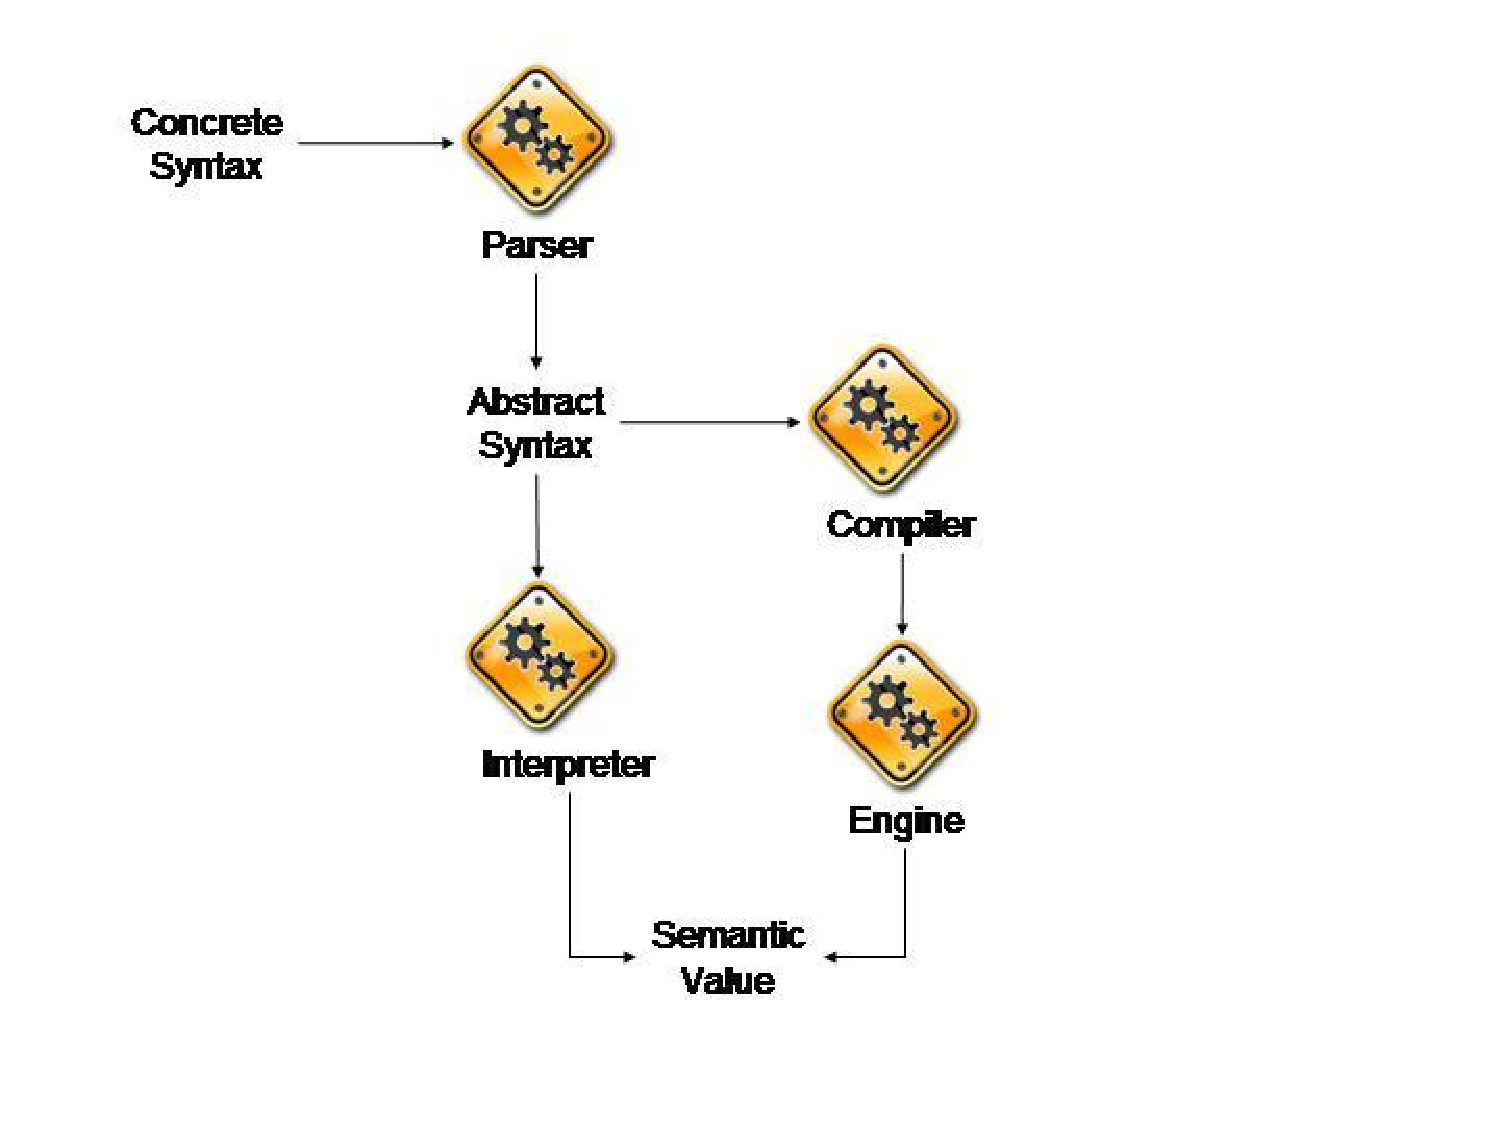
\includegraphics[width=12cm]{XMF/XOCL/Images/Evaluation.pdf}

\caption{Evaluation Process\label{fig:Evaluation-Process}}

\end{center} 
\end{figure}


An element is performable if it can be requested to do two tasks:
compile itself to a sequence of machine instructions and evaluate
itself to produce an element. In many ways these two tasks are similar
since compilation is translation from an element in one language to
an element in another; the instructions in the machine language can
each be asked to evaluate themselves. In order to design and develop
language constructs it is important to understand how to process syntax;
this section describes how XMF represents syntax and the various ways
of transforming and evaluating syntax.

Figure \ref{fig:Evaluation-Process} is an overview of the key syntax
processes. Processing starts with concrete syntax which is represented
as a sequence of characters. The characters may originate from a variety
of sources including files, strings or typed at a keyboard. A parser
is a processing engine that transforms a sequence of characters into
data elements; the data elements are referred to as abstract syntax.

Once syntax is represented in data, it can be processed in many different
ways. It can be transformed from one representation to another. It
can be analysed to see if it contains any errors. It can be executed
directly. The figure shows two different ways of evaluating syntax:
interpretation and compilation.

An interpreter is a program that takes another program as input and
runs it. An interpreter typically requires extra input to describe
the context of evaluation (for example the values for gobal variables
in the program). An interpreter is a program that itself must be written
in a language. The XOCL interpreter is written in XOCL and is easy
to extend.

A compiler is a program that translates a supplied program from a
source language to a target language. Typically the target language
has an interpreter which is somehow better than any interpreter for
the source language. For example the source language may not have
an interpreter or the target interpreter is much faster than any source
interpreter. In this case the XOCL compiler translates XOCL source
into XMF VM instructions for which there is an interpreter written
in Java. The XOCL compiler is written in XOCL and is easy to extend.

Every element that is to be used as syntax must implement the Performable
interface. Performable, requires that a syntax element knows how to
evaluate itself and how to compile itself. The interface is defined
as follows:

\begin{lstlisting}
Performable::compile(env,frame,isLast,saveSource)
// Produces a sequence of machine instructions.
// The env binds variable names that are currently
// in scope to type descriptors. The frame is an
// integer describing how many enclosing operations
// there are. isLast is true when there is nothing 
// further to perform. saveSurce is true when operations
// are to make theor source code available at run-time.
Performable::eval(target,env,imports)
// Evauates the element to produce a value. The target
// is the value of 'self' during evaluation. The 
// environment associates variable names with values.
// The imports are a sequence of imported name spaces.
Performable::FV()
// Returns a set of the free variables in the
// receiver.
Performable::maxLocals()
// Returns the maximum number of loal variables that
// is required in order to evaluate the receiver.
Performable::pprint(out,indent)
// Writes a textual version of the syntax to the
// output channel using indent as the current level
// of indentation after newlines.
\end{lstlisting}
Any new syntax should implement the Performable interface. Fortunately,
it is unusual to have to define all of this interface in practice
because sub-classes of Performable such as XOCL::Sugar shield the
user from the details. However, the following implementation of XOCL::While
shows how to implement a complete interface.

The instructions produced by compiling a while-loop involve skip-instructions.
The class While is a sub-class of Performable with performable attributes
for the while-test and the while-body:

\begin{lstlisting}
context While
  @Operation compile(env,frame,isLast,saveSource)
    let testCode = test.compile(env,frame,false,saveSource);
        bodyCode = body.compile(env,frame,false,saveSource);
        testLabel = Compiler::newLabel();
        endLabel = Compiler::newLabel() then
        returnValue = Compiler::labelInstrs(Seq{PushTrue()},endLabel)
    in Compiler::labelInstrs(testCode,testLabel) + 
       Seq{SkipFalse(endLabel)} + 
       bodyCode + 
       Seq{Pop()} + 
       Seq{SkipBack(testLabel)} + 
       returnValue
    end
  end
\end{lstlisting}
Given the above definition of compile for while-loops, XMF is able
to compile any file that contains a while-loop as part of the source
code. When the source file is compiled, the text is parsed and each
occurrence of concrete syntax for a while-loop is synthesized into
an instance of the class XOCL::While. The resulting syntax for the
complete file is then compiled. As part of the compilation, the while-loop
will perform the operation defined above and return the sequence of
instructions. The complete sequence of instructions for the whole
file is then written out as a binary file. The binary file is read
in at a later stage and the instructions are evaluated (either directly
when the file is read in or via the call of an operation defined in
the file).

Not all occurrences of a while-loop need to be compiled before they
can be performed. Expressions typed at the top-level of XMF are not
compiled, they are parsed to produce syntax objects and then evaluated.
It is also possible to evaluate the source code in a file directly
without having to compile it. The definition of eval for a while-loop
is given below:

\begin{lstlisting}
context While
  @Operation eval(target,env,imports)
    @While test.eval(target,env,imports) do
      body.eval(target,env,imports)
    end
  end
\end{lstlisting}
Although this definition seems at first to be self-referential (while
defined in terms of while), it is important to state that it is a
compiled operation and therefore the use of while in the body of the
operation is compiled using the definition of compile given above.
The key feature to note about the definition of eval is that the test
and body of the while-loop are evaluated using their own definitions
for eval.

A free variable is one that is used by a perfomable element, but which
is not locally defined by that element. In order to support compilation,
each performable elment must define FV. Since a while-loop does not
make direct reference to variables, the free variables are the union
of those for the test and body:

\begin{lstlisting}
context While
  @Operation FV():Set(String)
    test.FV() + body.FV()
  end
\end{lstlisting}
The opposite of free variables are bound variables. Again, in order
to support compilation it is necessary for the compiler to work out
how much local storage a performable element requires. Local variables
are introduced (for example) by a let-expression. A while-loop does
not directly introduce any local variables, but the test and body
might:

\begin{lstlisting}
context While
  @Operation maxLocals():Integer
    test.maxLocals().max(body.maxLocals())
  end
\end{lstlisting}
Finally, if the compiler is instructed to associate the source code
with each compiled operation, each element in the body of an operation
must be able to translate itself into a textual representation. This
is implemented for While as follows:

\begin{lstlisting}
context While
  @Operation pprint(out,indent)
    format(out,"@While ");
    test.pprint(out,indent);
    format(out," do~%~V",Seq{indent + 2});
    body.pprint(out,indent + 2);
    format(out,"~%~Vend",Seq{indent})
  end
\end{lstlisting}
While is a fairly simple example of a performable element. Here is
the complete implementation of a let-expression to give a :

\begin{lstlisting}
context Let
  @Operation compile(env,frame,isLast,saveSource)
    let valueCode = bindings->reverse->collect(b |
          b.value.compile(env,frame,false,saveSource))->flatten;
        letEnv = env.allocateLocals(bindings.name),env.maxLocal())
    in valueCode + 
       // Generate SETLOC instructions...
       letEnv.setLocalsCode(bindings.name) + 
       body.compile(letEnv,frame,isLast,saveSource)
    end
  end
context Let
  @Operation eval(target,env,imports)
    let newEnv = bindings->iterate(b e = env |
      e.bind(b.name,b.value.eval(target,env,imports)))
    in body.eval(target,newEnv,imports)
    end
  end
context Let
  @Operation FV():Set(String)
    bindings->iterate(binding FV = body.FV() - bindings.name->asSet |
      FV + binding.value.FV())
   end
context Let
  @Operation maxLocals():Element
    let valueMaxLocals = bindings->collect(b |
          b.value.maxLocals())->max;
        bindingMaxLocals = bindings->size;
        bodyMaxLocals = body.maxLocals()
    in valueMaxLocals.max(bindingMaxLocals + bodyMaxLocals)
    end
  end
context Let
  @Operation pprint(out,indent)
    format(out,"let ");
    if bindings.isKindOf(Seq(Element))
    then
      @For b in bindings do
        b.pprint(out,indent + 4);
        if not isLast
        then format(out,";~%~V",Seq{indent + 4})
        else format(out,"~%~V",Seq{indent})
        end
      end
    else bindings.pprint(out)
    end;
    format(out,"in ");
    body.pprint(out,indent + 3);
    format(out,"~%~Vend",Seq{indent})
  end
\end{lstlisting}
Defining new syntax classes in XMF requires two things to be associated
with the class: it must be a sub-class of Performable and therefore
implement the Performable interface as described in this section; it
must have a concrete syntax. Concrete syntaxes are defined in terms
of a grammar that synthesizes an instance of the syntax class. Concrete
syntaxes and grammars are the subject of the next chapter. 

The class defining the Object Command Language are defined in section
\ref{sec:OCL-Syntax-Classes}.

Fortunately, it is not usually necessary to define the complete Performable
interface for each new syntax class. This is because a new syntax
class can be defined in terms of a translation to existing syntax
classes that already implement the interface. This process is called
desugaring and is covered in section \ref{sec:Sugar-and-Expressions}.
Desugaring involves trnslating from one abstract syntax to another.
A useful technology to do this is quasi-quotes and this is the subject
of the next section.


\section{Quasi-Quotes and Lifting}

Suppose that we have a requirement for a new syntax for an until-loop.
An until-loop has the usual semantics and the syntax class has a body
and a test, both of which are performable. The syntax class Until
can fully implement the Performable interface, however, there is sufficient
syntax constructs in XOCL to support until-loops in terms of while-loops.
A traslation can be defined as follows:

\begin{lstlisting}
context Until
  @Operation translateToWhile(body,test)
    Order(body,While(test,body))
  end
\end{lstlisting}
The translateToWhile operation simply constructs instances of the
classes Order and While, supplying the appropriate body and test.
With larger syntax translations it becomes difficult to work with
target elements when they are directly constructed as instances of
the syntax classes. The reason is that we are used to seeing syntax
in concrete terms, not as instances of abstract classes. Worse still,
there are actually two uses of syntax in the body of translateToWhile:

\begin{enumerate}
\item The concrete syntax of object construction.
\item The abstract syntax of a command followed by a while-loop.
\end{enumerate}
When examples get a little larger than the one above, these issues
become very confusing. XMF provides technology to address this issue:
quasi-quotes. Quasi-quotes provide a means to construct syntax templates.
The body of transateToWhile can be viewed as a syntax template: the
fixed parts of the template are the ordering and the while-loop; the
variable parts are the supplied body and test. Quasi-quotes allow
the variable parts to be dropped into the fixed parts whih are expressed
using \emph{concrete syntax}. Here is the same operation using quasi-quotes:

\begin{lstlisting}
context Until
  @Operation translateToWhile(body,test)
    [| <body>; 
       @While <test> do 
         <body> 
       end
    |]
  end
\end{lstlisting}
The quotes are {\tt [|} and {\tt |]} surrounding concrete syntax. Within the
concrete syntax, code can be dropped in by surrounding the expressions
producing the code using {\tt <} and {\tt >}. In this case the expressions producing
the code are variables: body and test, but in principle the expressions
inside {\tt <} and {\tt >} can be anything that returns a performable element.

A typical pattern that occurs when working with syntax involves a
sequence of performable elements. Consider translating a sequence
of elements to produce a single expression that performs each expression
in order:
\begin{lstlisting}
@Operation orderCommands(commands:Seq(Performable))
  commands->iterate(command ordered = [| null |] |
    [| <ordered>; <command> |])
end
\end{lstlisting}
Translating syntax often involves the introduction and subsequent
reference of local variables. Introduction of local variables is typically
done via let-expressions and via operation arguments. This is easily
done using quasi-quotes, so long as you remember that variable names
are strings in let-bindings and operation arguments but variable references
are always done using the syntax class OCL::Var. Consider translating
a variable name, a classifier expression and a body expression into
an operation that checks the type of a supplied value, something like:

\begin{lstlisting}
@GuardedOp name(arg:type)
  body
end
\end{lstlisting}
is just like a normal operation except that the type of the value
supplied as arg is dynamically checked. The following translation
produces a normal operation and inserts the check:

\begin{lstlisting}
@Operation guardedOp(name:String,
                     arg:String,
                     type:Performable,
                     body:Performable)
  [| @Operation <name>(<arg>)
       if <Var(arg)>.isKindOf(<type>)
       then <body>
       else <Var(arg)>.error("Not of type " + <type>.toString())
       end
     end
  |]
end
\end{lstlisting}
Suppose that each a syntax construct allows the slots of an object
to be implicitly bound to variables, equivalent to a with-statement
in Pascal. Each variable is introduced using a let-expression:

\begin{lstlisting}
@Operation translateWith(object:Performable,
                         class:Class,
                         body:Performable)
  class.allAttributes()->iterate(a exp = body |
    let name = a.name().toString()
    in [| <name> = <object>.<name> in <exp> end |]
    end
  )
end
\end{lstlisting}
A problem with the translateWith translation is that the object expression
is performed many times. It is usual to introduce a local variable
for the value so that it is performed once. Also, suppose that the
with-translation is to be extended to put the values of the let-bound
variables back into the object at the end of the body:

\begin{lstlisting}
@Operation translateWith(object:Performable,
                         class:Class,
                         body:Performable)
  let A = class.allAttributes() then
      updateSlots = A->iterate(a exp = [| withResult |] |
        let name = a.name().toString()
        in [| withObject.<name> := <Var(name)>; <exp> |]
        end
      ) then
      completeBody = [| let withResult = <body> 
                        in <updateSlots> 
                        end |]
  in  [| let withObject = <object>
         in <A->iterate(a exp = completeBody |
               let name = a.name().toString()
               in [| let <name> = withObject.<name> 
                     in <exp> 
                     end |]
               end
            )>
         end
       |]
  end
end
\end{lstlisting}
Support that Point is a class with slots for the x and y position
in a diagram. A node is to be moved by dx and dy and will return the
new position as a pair:

\begin{lstlisting}
 translateWith(
   [| node.position |],
   Point,
   [| x := x + 1; y := y + 1; Seq{x,y} |])
\end{lstlisting}
The resulting performable element is pprinted as follows:

\begin{lstlisting}
let withObject = node.position
in let x = node.position.x
   in let y = node.position.y
      in let withResult = x := x + 1;
                          y := y + 1;
                          Seq{x,y}
         in withObject.x := x;
            withObject.y := y;
            withResult
         end
      end
   end
end
\end{lstlisting}
